%
% geraden.tex
%
% (c) 2018 Prof Dr Andreas Müller, Hochschule Rapperswil
%
\section{Geraden}
\rhead{Geraden}
\begin{figure}
\begin{center}
\begin{tabular}{ccc}
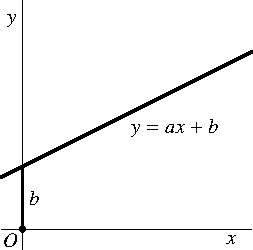
\includegraphics{images/v-6}&%
\qquad\qquad\qquad&
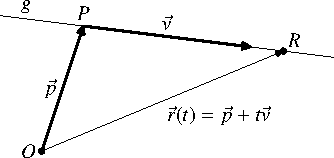
\includegraphics{images/v-7}%
\end{tabular}
\end{center}
\caption{Gerade in der Ebene (links) und Parametrisierung von Geraden im
Raum (rechts) \label{image-gerade}}
\end{figure}
Eine Gerade in einem Koordinatensystem in der Ebene kann durch eine
Gleichung der Form
\[
y=ax+b
\]
beschrieben werden (Abbildung~\ref{image-gerade}).
Die Gleichung hat als Lösungsmenge die Punkte
$(x,y)$, die auf einer Geraden der Steigung $a$ durch den Punkt $(0,b)$
liegen.
Der Nachteil dieser Darstellung ist, dass sich Geraden parallel zur $y$-Achse
damit nicht abbilden lassen.
Solche Geraden haben die Gleichung $x=c$, sie haben
``unendlich'' grosse Steigung.
Eine weitere Schwierigkeit besteht im Raum, wo noch eine weiter Koordinate
festzulegen ist.
Auch diese ist mit einer einzigen Gleichung nicht möglich.
Wir benötigen daher eine neue Form der Geradengleichung, welche für beliebige
Geraden in beliebigen Richtungen durch beliebige Punkte in beliebigen Räumen
unabhängig von der Dimension funktionieren.

\subsection{Parameterdarstellung}
\index{Parameterdarstellung!einer Gerade}
Die Punkte einer Geraden entstehen dadurch, dass ein Ausgangspunkt um
variable Längen in immer die gleiche Richtung verschoben wird.
Dies übersetzen wird jetzt in die Vektorsprache.
Eine Gerade wird also beschrieben durch
\begin{itemize}
\item einen Ausgangspunkt, oder seinen Ortsvektor $\vec p$.
Dieser Vektor heisst oft auch {\em Stützvektor}.
\index{Stutzvektor@Stützvektor}
\item Von diesem Ausgangspunkt aus müssen Strecken in eine bestimmte
Richtung angesetzt werden, dazu brauchen wir einen Vektor, wir nennen ihn
$\vec v$, den {\em Richtungsvektor}.
\index{Richtungsvektor}
\item Die angesetzten Vektoren sind von variabler Länge, es braucht also
einen Parameter, den wir $t\in \mathbb R$ nennen, mit welchem $\vec v$
multipliziert wird.
\end{itemize}
Auf diese Weise erreichen wir die Punkte $\vec r$ der Gerade mit Hilfe
einer Addition:
\[
\vec r(t)=\vec p+t\vec v,
\]
Abbildung~\ref{image-gerade}, rechts.
Mit dieser Definition lassen sich gewisse Grundaufgaben bereits lösen.

\begin{beispiel}
Man finde die Parameterdarstellung der Geraden durch die Punkte
$A=(3,1,4)$ und $B=(1,5,9)$.

\smallskip

{\parindent 0pt
Dazu} braucht man einen Vektor, der die Funktion von $\vec p$ übernehmen
kann, wir verwenden $\overrightarrow{OA}$ dafür, und als
Richtungsvektor können wir $\overrightarrow{AB}$ verwenden.
Damit wird die Geradengleichung
\begin{equation}
\vec r(t) =
\begin{pmatrix}3\\1\\4 \end{pmatrix}
+t
\begin{pmatrix}-2\\4\\5\end{pmatrix}.
\label{pigerade}
\end{equation}
\end{beispiel}

\subsubsection{Geht eine Gerade durch einen Punkt?}
Gegeben ist die Gerade durch $\vec p$ mit Richtungsvektor $\vec v$.
Geht die
Gerade durch den Punkt $\vec s$? Offenbar müssen wir herausfinden, ob es
einen Wert des Parameters $t$ gibt, für den der Geradenpunkt mit $\vec s$
identisch ist, also
\[
\vec s = \vec p + t\vec v.
\]
Diese Vektorgleichung ist genau genommen ein Gleichungssystem für die einzelnen
Komponenten
\[
\begin{pmatrix}
s_1\\s_2\\s_3
\end{pmatrix}
=
\begin{pmatrix}
p_1\\p_2\\p_3
\end{pmatrix}
+t
\begin{pmatrix}
v_1\\v_2\\v_3
\end{pmatrix}
\qquad
\Rightarrow
\qquad
\begin{aligned}
s_1&=p_1+tv_1\\
s_2&=p_2+tv_2\\
s_3&=p_3+tv_3
\end{aligned}
\]
Dieses Gleichungssystem mit drei Gleichungen aber nur einer Unbekannten wird
meistens nicht lösbar sein.
Aber es gilt natürlich die übliche Alternative
für lineare Gleichungssysteme:
\begin{itemize}
\item Es kann keine Lösungen geben: Dieser Fall tritt ein, wenn die Gerade
an dem Punkt vorbei geht.
\item Es kann unendlich viele Lösungen geben: Dieser Fall tritt ein, wenn
$\vec v=0$ ist und $\vec p=\vec s$.
Dann ``bleibt'' der Punkt $\vec r(t)$
immer am Ort $\vec p$, welcher identisch ist mit dem gesuchten Punkt $\vec s$.
\item Es kann genau eine Lösung geben: falls $\vec v\ne 0$ und der Punkt auf der
Geraden liegt, gibt es genau einen Parameterwert, für den der Punkt
getroffen wird.
\end{itemize}
Den Parameterwert im Fall 3 kann man zum Beispiel finden, indem man eine
der Gleichungen auswählt, in der der $v_i$-Koeffizient nicht $0$ ist
Diese Gleichung löst man nach $t$ auf.
Falls $v_1\ne 0$ heisst das
\[
t=\frac{s_1-p_1}{v_1}.
\]
Durch Einsetzen in die anderen Gleichungen kann man anschliessend auch überprüfen,
ob die Gerade tatsächlich durch den Punkt geht.

\begin{beispiel} Welcher der Punkte $U=(5,-3,-1)$ und $V=(7,-7,-7)$
liegt auf der Geraden (\ref{pigerade})?

\smallskip

{\parindent 0pt Um zu testen},
ob die Gerade durch den Punkt mit Ortsvektor $\vec u$
geht, muss man versuchen, die Gleichung
\[
\begin{pmatrix}3\\1\\4 \end{pmatrix}
+t
\begin{pmatrix}-2\\4\\5\end{pmatrix}
=\vec u
\]
zu lösen.
Für die beiden Ortsvektoren $\vec u$ und $\vec v$
bedeutet das
\begin{align*}
t_1
\begin{pmatrix}-2\\4\\5\end{pmatrix}
+
\begin{pmatrix}3\\1\\4 \end{pmatrix}
&=
\begin{pmatrix}5\\-3\\-1\end{pmatrix}
&
\qquad
t_2
\begin{pmatrix}-2\\4\\5\end{pmatrix}
+
\begin{pmatrix}3\\1\\4 \end{pmatrix}
&=
\begin{pmatrix}7\\-7\\-7\end{pmatrix}
\\
t_1
\begin{pmatrix}-2\\4\\5\end{pmatrix}
&=
\begin{pmatrix}5\\-3\\-1\end{pmatrix}
-
\begin{pmatrix}3\\1\\4 \end{pmatrix}
=
\begin{pmatrix}2\\-4\\-5 \end{pmatrix}
&
\qquad
t_2
\begin{pmatrix}-2\\4\\5\end{pmatrix}
&=
\begin{pmatrix}7\\-7\\-7\end{pmatrix}
-
\begin{pmatrix}3\\1\\4 \end{pmatrix}
=
\begin{pmatrix}4\\-8\\-11\end{pmatrix}
\\
t_1&=-1,&t_2&:\text{keine Lösung.}
\end{align*}
Es folgt, dass $U$ auf der Geraden liegt, $V$ aber nicht.
\end{beispiel}

\subsubsection{Geschwindigkeitsvektor}
\index{Geschwindigkeitsvektor}
Interpretiert man $t$ als die Zeit, dann bewegt sich ein Punkt auf der Geraden in
einer Sekunde um $\vec v$, dieser Vektor stellt also die Geschwindigkeit
des Punktes dar.
Die Parameterdarstellung der Geraden ist also auch eine
Beschreibung einer gleichförmigen Bewegung.

\subsubsection{Spezialfall Dimension 2}
In Dimension 2 wird die Geradengleichung zu
\[
\begin{pmatrix}
x\\y
\end{pmatrix}
=
\begin{pmatrix}
x_0\\y_0
\end{pmatrix}
+t
\begin{pmatrix}
v_x\\v_y
\end{pmatrix}
\qquad
\Rightarrow
\qquad
\begin{aligned}
x&=x_0+tv_x\\
y&=y_0+tv_y
\end{aligned}
\]
Falls $v_x\ne 0$ (was gleichbedeutend ist damit, dass die Gerade
nicht parallel zur $y$-Achse ist, kann man die erste Gleichung nach
$t$ auflösen:
\[
t = \frac{x-x_0}{v_x}
\]
und in die zweite Gleichung einsetzen:
\[
y=y_0+
\frac{x-x_0}{v_x}v_y
=
y_0+\frac{v_y}{v_x}(x-x_0)
=
y_0-mx_0 +mx
=
mx+(y_0-mx_0)=mx+b
\]
Es entsteht also eine Geradengleichung der Art, wie sie uns schon früher
bekannt war.
Der Quotient $m=\frac{v_y}{v_x}$
ist offenbar die Steigung der Geraden, $y_0-mx_0$ ist der Achsabschnitt.
Die Vektorschreibweise ist jedoch vorteilhaft, weil sie keine der
Koordinaten besonders hervorhebt, und damit auch Spezialfälle wie
die $y$-Achse besser darstellen kann\footnote{In diesem Spezialfall ist
$v_x=0$, also ist die Steigung $m=\frac{v_y}{v_x}$ nicht definiert.}.

\subsection{Schnittpunkt von zwei Geraden}
\index{Schnittpunkt zweier Geraden}
Seien jetzt zwei Geraden gegeben, also zwei Ausgangspunkte $\vec p_1$ und
$\vec p_2$ und zwei Richtungsvektoren $\vec v_1$ und $\vec v_2$.
Haben die beiden Geraden einen Schnittpunkt?
Jede der Geraden ist durch die Parameterdarstellung
$\vec r=\vec p_1+t\vec v_1$
bzw.~$\vec r=\vec p_2+t\vec v_2$
gegeben.
Wir können natürlich nicht annehmen, dass der Schnittpunkt,
wenn es ihn überhaupt gibt, von beiden Geraden mit dem gleichen Parameterwert
$t$ erreicht wird.
Wir müssen also zwei verschiedene Parameterwerte $t$
und $s$ finden, die eingesetzt in die beiden Geradengleichungen zum gleichen
Punkt führen, also:
\[
\vec p_1+t\vec v_1=\vec p_2+s\vec v_2,
\]
oder
\[
t\vec v_1-s\vec v_2=\vec p_2-\vec p_1.
\]
Dies ist ein Gleichungssystem mit zwei Unbekannten, für die Anzahl der Lösungen
gilt wieder die bekannte Alternative:
\begin{itemize}
\item Keine Lösungen: Die Geraden haben keinen Schnittpunkt, in der Ebene
kann dies zum Beispiel dadurch geschehen, dass die Geraden parallel sind.
Im Raum können die Geraden auch windschief sein.
In drei Dimensionen erhalten wir drei Gleichungen mit nur einer Unbekannten,
dieses System wir normalerweise nicht lösbar sein.
\item Unendlich viele Lösungen: die Geraden sind deckungsgleich
\item Genau eine Lösung: es gibt einen wohldefinierten Schnittpunkt.
\end{itemize}
Gelöst werden kann das Gleichungssystem natürlich mit den Standardverfahren
für lineare Gleichungssysteme.

\begin{beispiel}
Man finde den Schnittpunkt der Geraden $g_1$ und $g_2$ mit den
Parameterdarstellungen
\begin{align*}
g_1:
\vec r
&=t\begin{pmatrix}5\\6\\1\end{pmatrix}+\begin{pmatrix}0\\4\\2\end{pmatrix}
&
g_2:
\vec r
&=s\begin{pmatrix}5\\2\\4\end{pmatrix}+\begin{pmatrix}-15\\-6\\-7\end{pmatrix}
\end{align*}

\smallskip

{\parindent 0pt Durch}
Gleichsetzen erhält man ein Gleichungssystem mit drei Gleichungen
für die zwei Unbekannten $s$ und $t$:
\[
t\begin{pmatrix}5\\6\\1\end{pmatrix}
-s\begin{pmatrix}5\\2\\4\end{pmatrix}
=\begin{pmatrix}-15\\-6\\-7\end{pmatrix}
-\begin{pmatrix}0\\4\\2\end{pmatrix}
=\begin{pmatrix}-15\\-10\\-9\end{pmatrix}
\]
Lösung mit dem Gauss-Algorithmus ist
\begin{align*}
\begin{tabular}{|>{$}c<{$}>{$}c<{$}|>{$}c<{$}|}
\hline
5%
\begin{picture}(0,0)%
\color{red}\put(-3,4){\circle{12}}
\end{picture}%
&-5&-15\\
6&-2&-10\\
1%
\begin{picture}(0,0)%
\color{blue}\drawline(-8,-2)(-8,24)(2,24)(2,-2)
\end{picture}%
&-4&-9\\
\hline
\end{tabular}
&
\rightarrow
\begin{tabular}{|>{$}c<{$}>{$}c<{$}|>{$}c<{$}|}
\hline
1&-1&-3\\
0& 4%
\begin{picture}(0,0)
\color{red}\put(-3,4){\circle{12}}
\end{picture}%
& 8\\
0&-3%
\begin{picture}(0,0)
\color{blue}\drawline(-15,-2)(-15,10)(1,10)(1,-2)
\end{picture}%
&-6\\
\hline
\end{tabular}
\rightarrow
\begin{tabular}{|>{$}c<{$}>{$}c<{$}|>{$}c<{$}|}
\hline
1&-1%
\begin{picture}(0,0)%
\color{blue}\drawline(-15,10)(-15,-2)(1,-2)(1,10)
\end{picture}%
&-3\\
0& 1& 2\\
0& 0& 0\\
\hline
\end{tabular}
\rightarrow
\begin{tabular}{|>{$}c<{$}>{$}c<{$}|>{$}c<{$}|}
\hline
1& 0&-1\\
0& 1& 2\\
0& 0& 0\\
\hline
\end{tabular}
\end{align*}
Der Schnittpunkt ist $S=(-5,-2,1)$.
\end{beispiel}

